\documentclass[
a4paper
]{scrreprt}
\usepackage[ngerman]{babel}
\usepackage[utf8]{inputenc}
\usepackage{textcomp, expdlist, array, colortbl, xcolor}
\usepackage[pdftex]{graphicx}
\usepackage[TS1, T1]{fontenc}
\usepackage{palatino} % Schriftart
\usepackage{parskip} %Erste Zeile eines Paragrafen nicht einrücken

\usepackage{listings}
\usepackage{color}
\usepackage{xcolor}

% Snippets settings
\lstset{language=C++,
	basicstyle=\ttfamily,
	keywordstyle=\color{blue}\ttfamily,
	stringstyle=\color{red}\ttfamily,
	commentstyle=\color{magenta}\ttfamily,
	morecomment=[l][\color{magenta}]{\#}
}


\begin{document}
\sffamily % Whole document sans-serif


% Titelseite
\begin{titlepage}
\centering

\includegraphics[width=0.8\textwidth]{./images/logo_hska.png}\par\vspace{1cm}
\vspace{1cm}

{\scshape\Large Systemnahes Programmieren\par}
\vspace{1.5cm}

{\huge\textbf{Compiler}\par}
\vspace{2cm}

{\Large\itshape Timo Blust, 48594\par}
{\Large\itshape Gennadi Eirich, 50629\par}
{\Large\itshape Tim Essig, 49683\par\par}
\vspace{2cm}

{\Large\itshape Gruppe 17 (WS 15/16)\par}

\vfill

% Bottom of the page
{\large \today\par}
\end{titlepage}


% Inhaltsverzeichnis
\tableofcontents

% Scanner
\chapter{Scanner}
\section{State Machine}
Da im zweiten Teil des Kompiler-Projekts neue Schlüsselworter hinzukommen, muss zunächst der Token Scanner (der Verwalter der Automaten) angepasst werden. Durch die modulare Struktur des Token Scanners ist dies jedoch mit geringem Aufwand möglich, da jedes Token (also auch jedes Schlüsselwort) einen eigenen Automaten besitzt.

Die Automaten für die neuen Schlüsselwörter    
\begin{lstlisting}     
  int
  else
  read
  write
\end{lstlisting}    
können mithilfe der statischen Funktion \lstinline{StateMachine::createString} generiert werden. Diese Funktion erzeugt einen Zustandsautomaten, welcher genau die übergebenen Strings akzeptiert. Der Automat für das Schlüsselwort \lstinline{else} wird zum Beispiel so erzeugt:
\begin{lstlisting}
StateMachine::createString(Token::KW_ELSE, 
                           new const char*[2]{ "ELSE", "else" }, 
                           2);
\end{lstlisting}

\begin{figure}
\centering
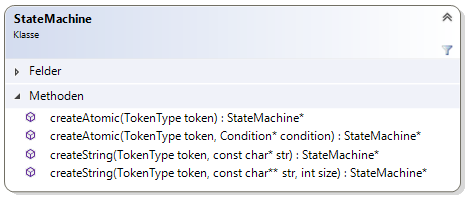
\includegraphics[width=0.8\textwidth]{./images/statemachine.png}
\caption{Vereinfachtes Klassendiagramm von StateMachine}
\end{figure}

\chapter{Parser}
Der Parser hat die Aufgabe, aus der Tokensequenz die der Scanner liefert, einen Strukturbaum zu erstellen, hierbei prüft er auch die syntaktische Korrektheit. Der Datenfluss ist wie folgt: Der Parser fordert die Tokens vom Scanner an. Der Parser führt nach der Erstellung des Strukturbauems ebenfalls einen Typenprüfung durch und generiert den Code für die VM.
\section{Parse Tree}
Der Parser hat die Aufgabe aus den Tokens, welche der Scanner liefert, einen ParseTree auf zu spannen.  Um dies umzusetzen schaut der Parser immer ein Token voraus, somit wird die Ableitung eindeutig. Der Parser startet mit dem Startsymbol \textit{PROG} und erzeugt von da ausgehen für jede erkannte Regel einen neuen Teilbaum.\\

\begin{figure}[htbp]
\centering
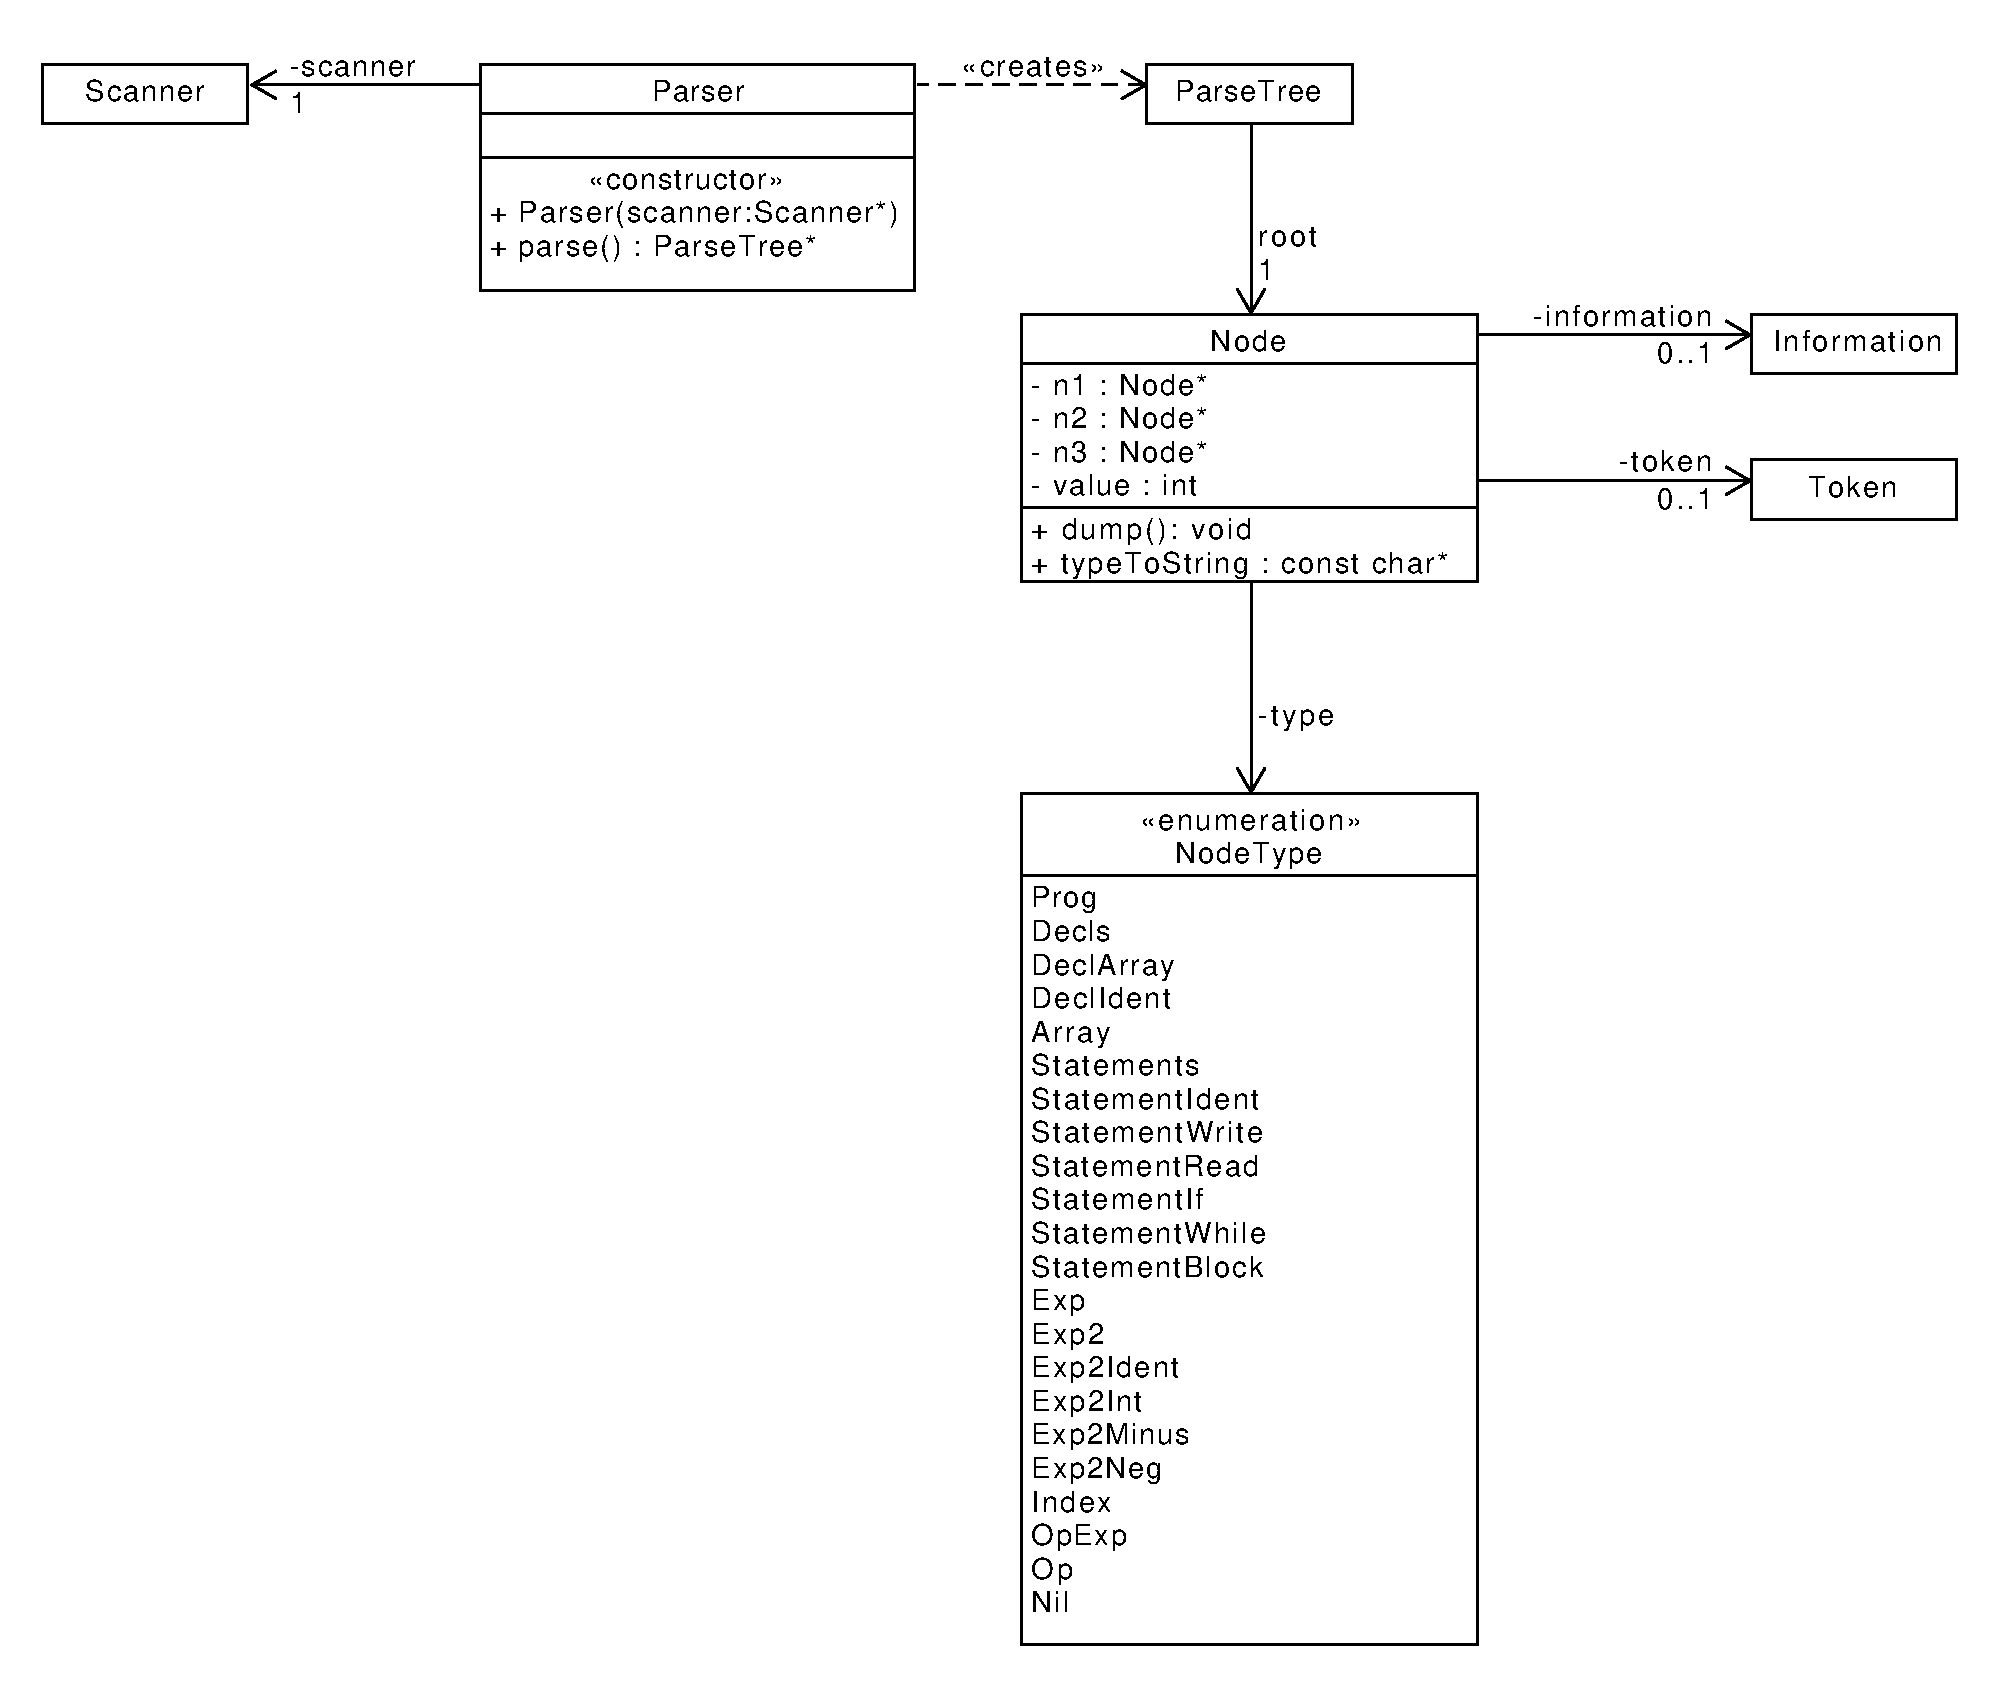
\includegraphics[width=\textwidth]{./diagramms/parser.pdf}
\caption{Klassendiagramm des ParseTree}
\label{parseTree}
\end{figure}


\section{Type Checking}
Nach der erfolgreichen Generierung des Parse Trees erolgt eine Typ-Prüfung. Hierbei wird geprüft, ob sämtliche Ausdrückte semantisch korrekt sind. Wird zum Beispiel ein Identifier mehrfach definiert (egal ob vom selben Typ oder verschiedenen Typen), ist es Aufgabe des Type Checks diesen Fehler zu ermittlen und zu melden.

Folgende Punkte werden während des Type Checks geprüft:
\begin{itemize}
\item Mehrfache Definition des gleichen Identifiers
\item Inkompatible Datentypen (z.B. einer Variable vom Typ Integer-Array wird ein Wert vom Typ Integer zugewiesen)
\item Verwendung von undefinierten Identifiern
\item Ungültige Länge in Arraydefinitionen (z.B. \lstinline{int[0] toSmall;})
\end{itemize}

Das Ablaufdiagramm in Abbildung \ref{TypeCheck1} und \ref{TypeCheck2} zeigt die Funktionsweise der Typ-Prüfung.

\begin{figure}[htbp]
\centering
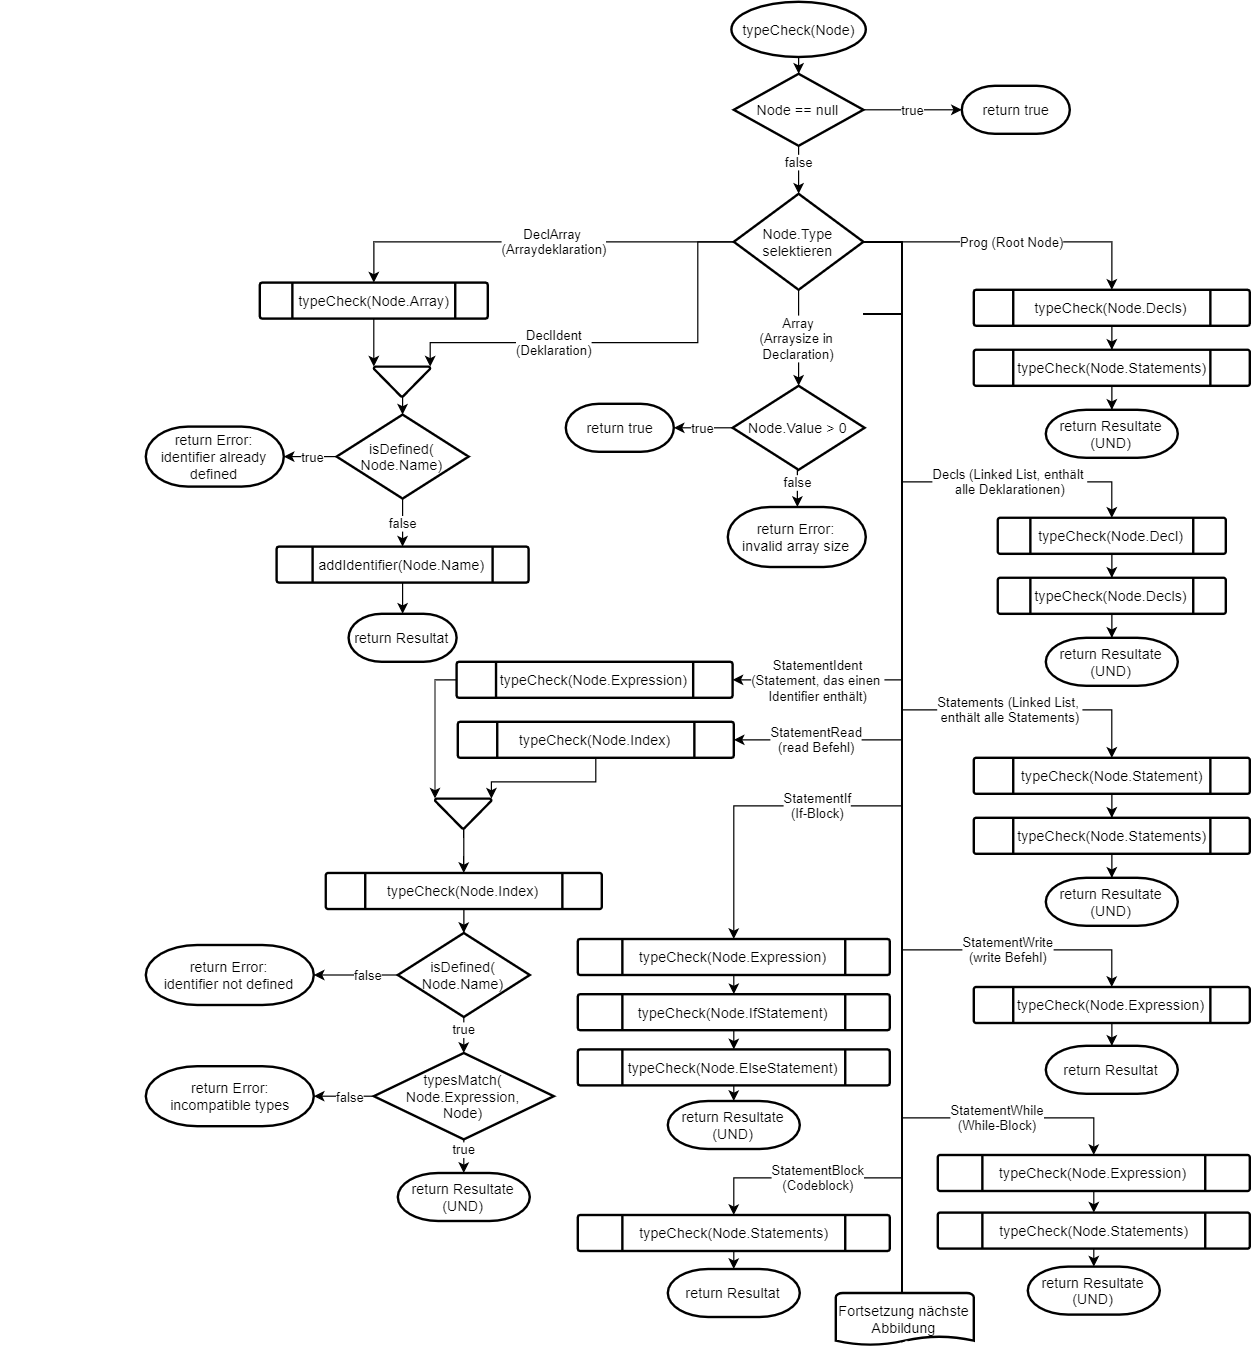
\includegraphics[width=\textwidth]{./images/TypeCheck1.png}
\caption{Ablaufdiagramm des Type Checks (Teil 1)}
\label{TypeCheck1}
\end{figure}

\begin{figure}[htbp]
\centering
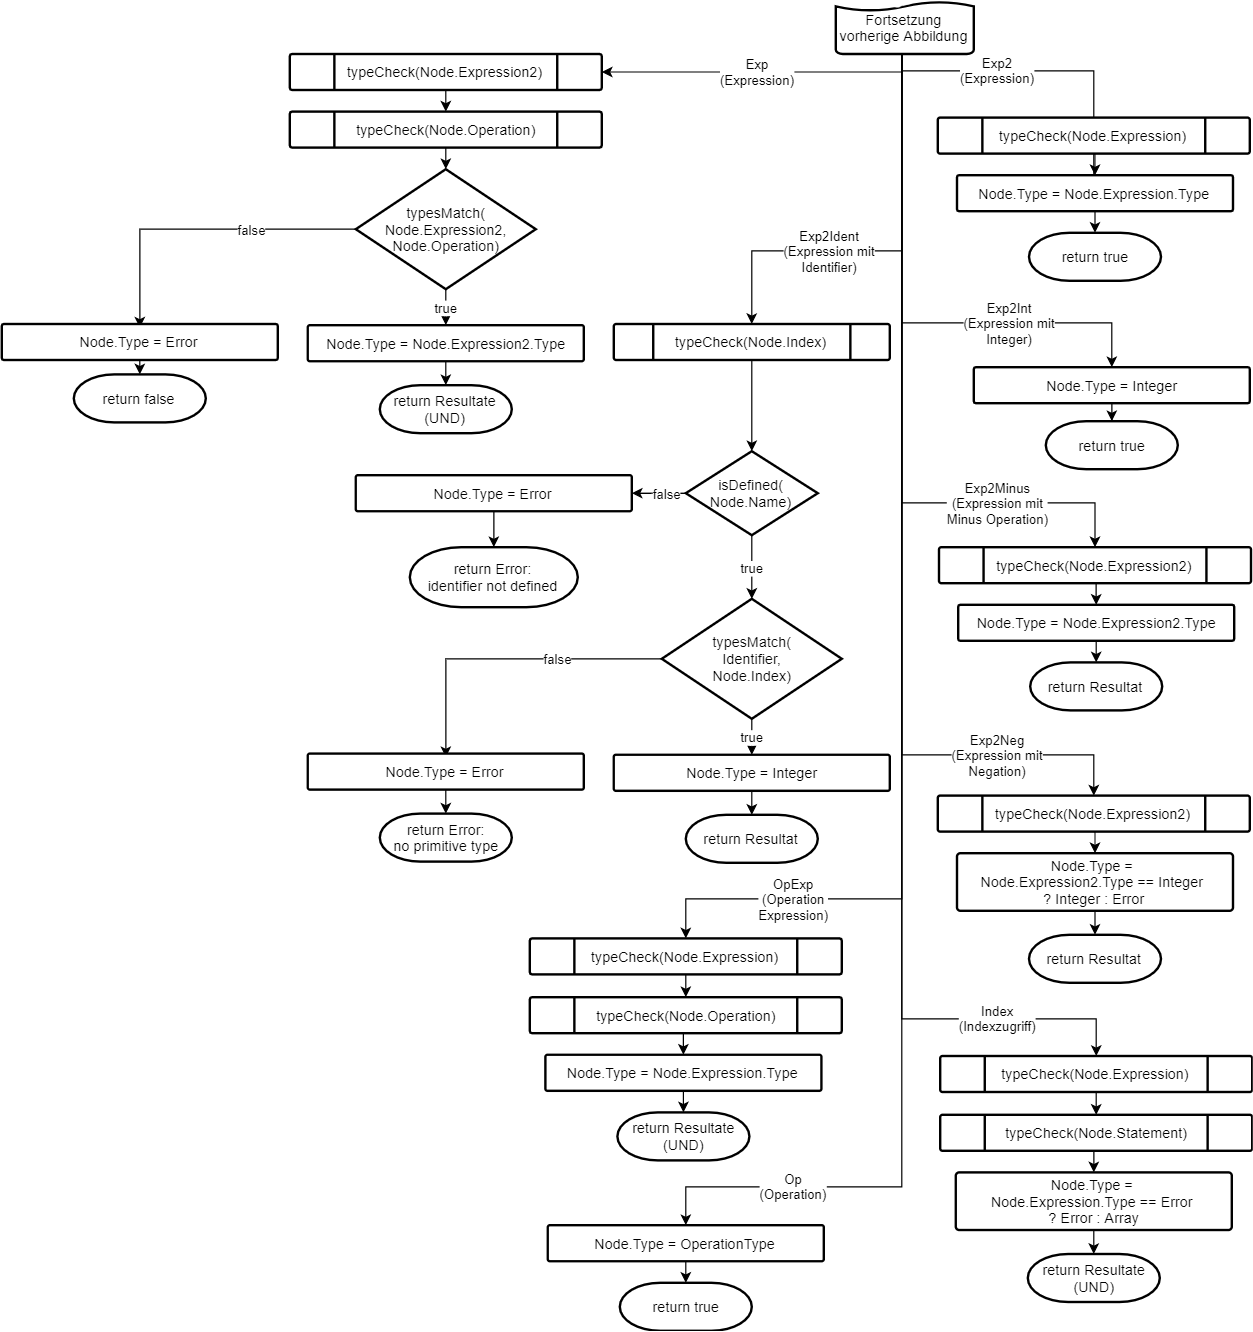
\includegraphics[width=\textwidth]{./images/TypeCheck2.png}
\caption{Ablaufdiagramm des Type Checks (Teil 2)}
\label{TypeCheck2}
\end{figure}


\section{Code Generation}
//TODO: Gena


\end{document}